
\section{Background}\vspace{3 mm}
\subsection{Unit Testing}
Unit testing is important part of software development. Unit testing is a software testing method that seeks to uncover new software bugs hidden at individual units of the software and it will be the first pass of testing as soon as individual building blocks of a big software is build.  Unit testing is a method by which individual units of source code, sets of one or more computer program modules together with associated control data, usage procedures, and operating procedures are tested to determine if they are fit for use.\\

There are many tools available to ease the unit testing process. Cunit a unit testing framework for C [1] is a tool which aids unit testing of C applications.  The CuTest [2] is another tool which is also used for unit testing C applications.\\

\subsection{SCSI}

SCSI (Acronym for Small Computer System Interface) is a collection of ANSI standards and proposed standards which define I/O busses primarily intended for connecting storage subsystems or devices to hosts through host bus adapters. Originally intended primarily for use with small (desktop and desk-side workstations) computers, SCSI has been extended to serve most computing needs, and is arguably the most widely implemented I/O control structure in use today.  SCSI Architecture Model (SAM) is an ANSI standard that defines the generic requirements and overall framework in which other SCSI standards are defined. \\

The first two SCSI standards (SCSI and SCSI-2) were all-in-one standards. They included everything from cables and connectors to protocols to command sets in one standard. The InterNational Committee for Information Technology Standards (INCITS) T10 Technical adopted a layered standards approach much like the International Organization for Standardization (ISO) Reference Model for networking standards. This approach divides SCSI into multiple layers of standards. The lowest layer deals with physical interfaces (also called transports). The next layer up deals with transport protocols usually directly associated with one physical transport standard. The top layer consists of command sets associated with specific devices such as disk drives or tape drives. \\

The image mentioned below is reproduced from T10 SAM specification depicts how the different standards of SCSI are layered in the SAM.  From the picture below, it can be seen that majority of the storage devices, whether  it is SAS, SATA, SCSI, FC,  iSCSI or the latest PCIe all are covered under the big umbrella of SCSI.\\

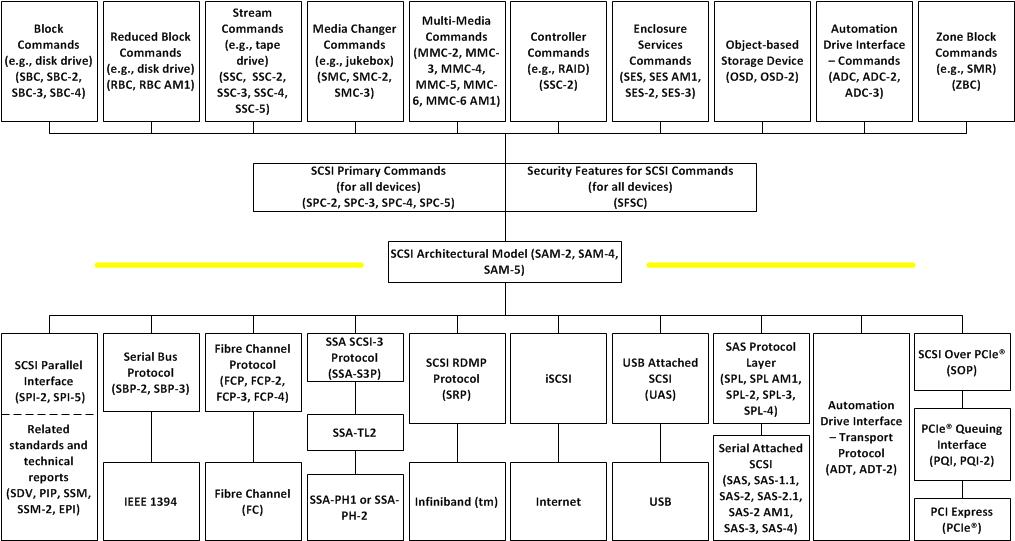
\includegraphics[scale=.6]
{SAM}

\subsection{Linux Kernel’s SCSI Device Driver Architecture} 

Layered SCSI architecture is mirrored in the software architecture as well. Operating systems use layered driver structures such as SCSI Common Access Method (CAM). This architecture has one or more class drivers that share one or more host bus adapter drivers. This allows both disk drives and tape drives to coexist on the same parallel SCSI bus. It also permits a disk class driver to control both parallel SCSI and Fiber Channel disk drives. This protects software investment as people migrate to newer physical interfaces.\\

The Linux kernel I/O subsystem consists of multiple layers of drivers.  The SCSI subsystem is part of the Linux I/O subsystem and handles majority of storage devices belong to different storage protocol family.  The Parallel SCSI (SPI), Fibre Channel (FC), Serial Attached Scsi (SAS) and Serial ATA (SATA) devices are managed by the SCSI subsystem of Linux kernel.   The SCSI subsystem is a layer between the File System Drivers and actual storage Host Bus Adapter (HBA) hardware. The SCSI subsystem itself is a layered architecture with three different layers of drivers (or kernel modules). The architecture of the I/O subsystem and SCSI subsystem are represented in the pictures below.\\

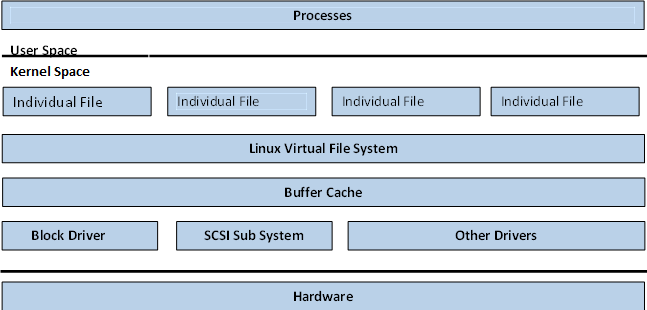
\includegraphics[scale=.9]
{fig2}

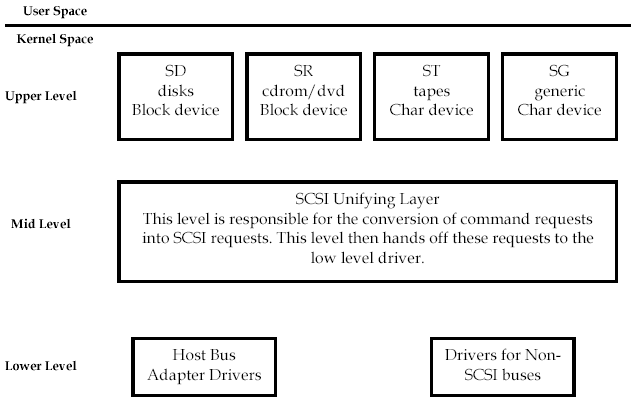
\includegraphics[scale=.9]
{fig3}


The SCSI subsystem in Linux consists of three layers namely Upper Level (ULD), Mid Level (SML) and Low Level (LLD).  The SCSI subsystem uses a three layer design with upper, mid, and low level layers. Every operation involving the SCSI subsystem (such as reading a sector from a disk) uses one driver at each of the 3 levels: one upper level driver, one lower level driver and the SCSI midlevel.\\

The SCSI upper level provides the interface between user space and the kernel, in the form of block and char device nodes for I/O and IOCTL. The low level contains drivers for specific hardware devices. In between is the SCSI midlevel, analogous to a network routing layer such as the IPv4 stack. \\

The SCSI midlevel routes a packet based data protocol between the upper levels device nodes and the corresponding devices in the lower level. It manages command queues, provides error handling and power management functions, and responds to I/O control (IOCTL) requests. The upper level and midlevel drivers are developed by Linux kernel SCSI developers.  There will be at least one type of upper level driver for a type of SCSI device. For example the SD driver handles all disk drives and the ST driver handles tape devices and similarly other upper level driver handles a particular type of device. The midlevel driver named scsi\_mod handles the entire house keeping activities like timing the SCSI requests and handling errors etc and it is a core for the SCSI driver model in Linux.  The midlevel driver also is maintained by Linux SCSI developers. \\

The low level drivers are the hardware specific driver and they translate the SCSI commands sent by the midlevel into the commands which can be understood by the hardware.  Hence the low level drivers are usually developed and maintained by hardware manufacturing companies. The Linux kernel community does rigorous code reviews before accepting driver code submission from the hardware vendor into kernel source tree.  \\

Considering the above, it will require a humongous work to develop one generic common unit testing frame work for all Linux kernel modules. Hence we decided to approach the problem in piece meal fashion.\\

As mentioned above, the SCSI subsystem is a major class of device drivers of the Linux operating system. It provides support for peripheral devices that support the SCSI interface, such as high performance hard drives. The code for the SCSI subsystem can be found in the ``drivers/scsi" directory of the source code distribution. SCSI support has been present in Linux since the first official release of the kernel in 1994. Like the rest of the kernel, the SCSI drivers are open source. However most of the low level drivers have been developed and then donated by the companies that developed the SCSI controllers themselves. That is, unlike much of the core of the Linux kernel, the original development of most of the low level driver code was performed within a company by full time developers, and not by the open source community. \\

One noteworthy feature of the SCSI subsystem is that it is designed and implemented as a strict three level architecture: the top and middle levels provide a set of unified and consistent commands for the kernel to control various drivers while the low-level drivers are concrete implementations of this functionality peculiar to the specifics of the particular hardware. Abstractly, the low-level drivers all implement the same functionality, such as hardware initialization, I/O handling, and error checking; they interact with the rest of the operating system only through the upper two levels.\\

The controlled interfaces between the low level and midlevel and most common functionalities between various low level drivers make low level driver (LLD) as in ideal candidate for unit testing using a generic unit test tool.  The unit testing of LLD also has similar limitation of other kernel modules.  Today to test a LLD, the test cases are executed from user space through the generic application interface available and requires whole stack. The LLD are developed by hardware vendors and testing of the LLD are typically done after integrating the driver into the complete stack and by running applications to execute the LLD functionalities from user space.  The application calls has to pass through all the layers above LLD to test a particular functionality of LLD this is an unnecessary overhead and nullifies the whole purpose of unit level testing. If there is any failure, lot of debug effort is required to isolate a fault at unit level.  Also testing a LLD interface thoroughly is not possible today as it is not standalone. Certain functionalities cannot be tested due to restrictions imposed by the upper levels.  For example there is an interface implemented by LLD named \textit{queuecommand}, the \textit{queuecommand} interface of an individual LLD will be invoked by the midlevel when it wants to send a new command to a hard drive. The LLD is expected to validate the command and return error when the command is sent to an unknown device.  But due to the reason that SML keeps track of only known devices, that condition can never be tested through SML.  If in future if the SML send a command to unknown device if LLD cannot capture that and return error it will results in failure of LLD.  \\

The Linux community recognizes the need for unit test tool for LLD as over the last 20 years, the    LLD code base is increased from 0 to 500 K but there is no available test tool for validating LLD before acceptance into kernel source tree. \\

Hence we are motivated to 
\begin{enumerate}
\item Port an application level unit test tool for C to kernel. 
\item Develop a Kernel module and associated applications to commonly test various interfaces of LLD by utilizing the unit test tools ported to kernel.
\end{enumerate}

Unit testing of LLD requires two different levels of testing.  One is to test the higher level interaction of the LLD (with SML or ULD) and the other is testing the hardware interaction.  Writing a common unit test module to hardware level is not really possible as the hardware interaction is in general is through proprietary interfaces provided by hardware vendors. So we will be limiting our efforts to unit testing of higher level interaction interfacing of LLD.\\



